\label{sec:chunk_flooding}
\begin{figure*}
  %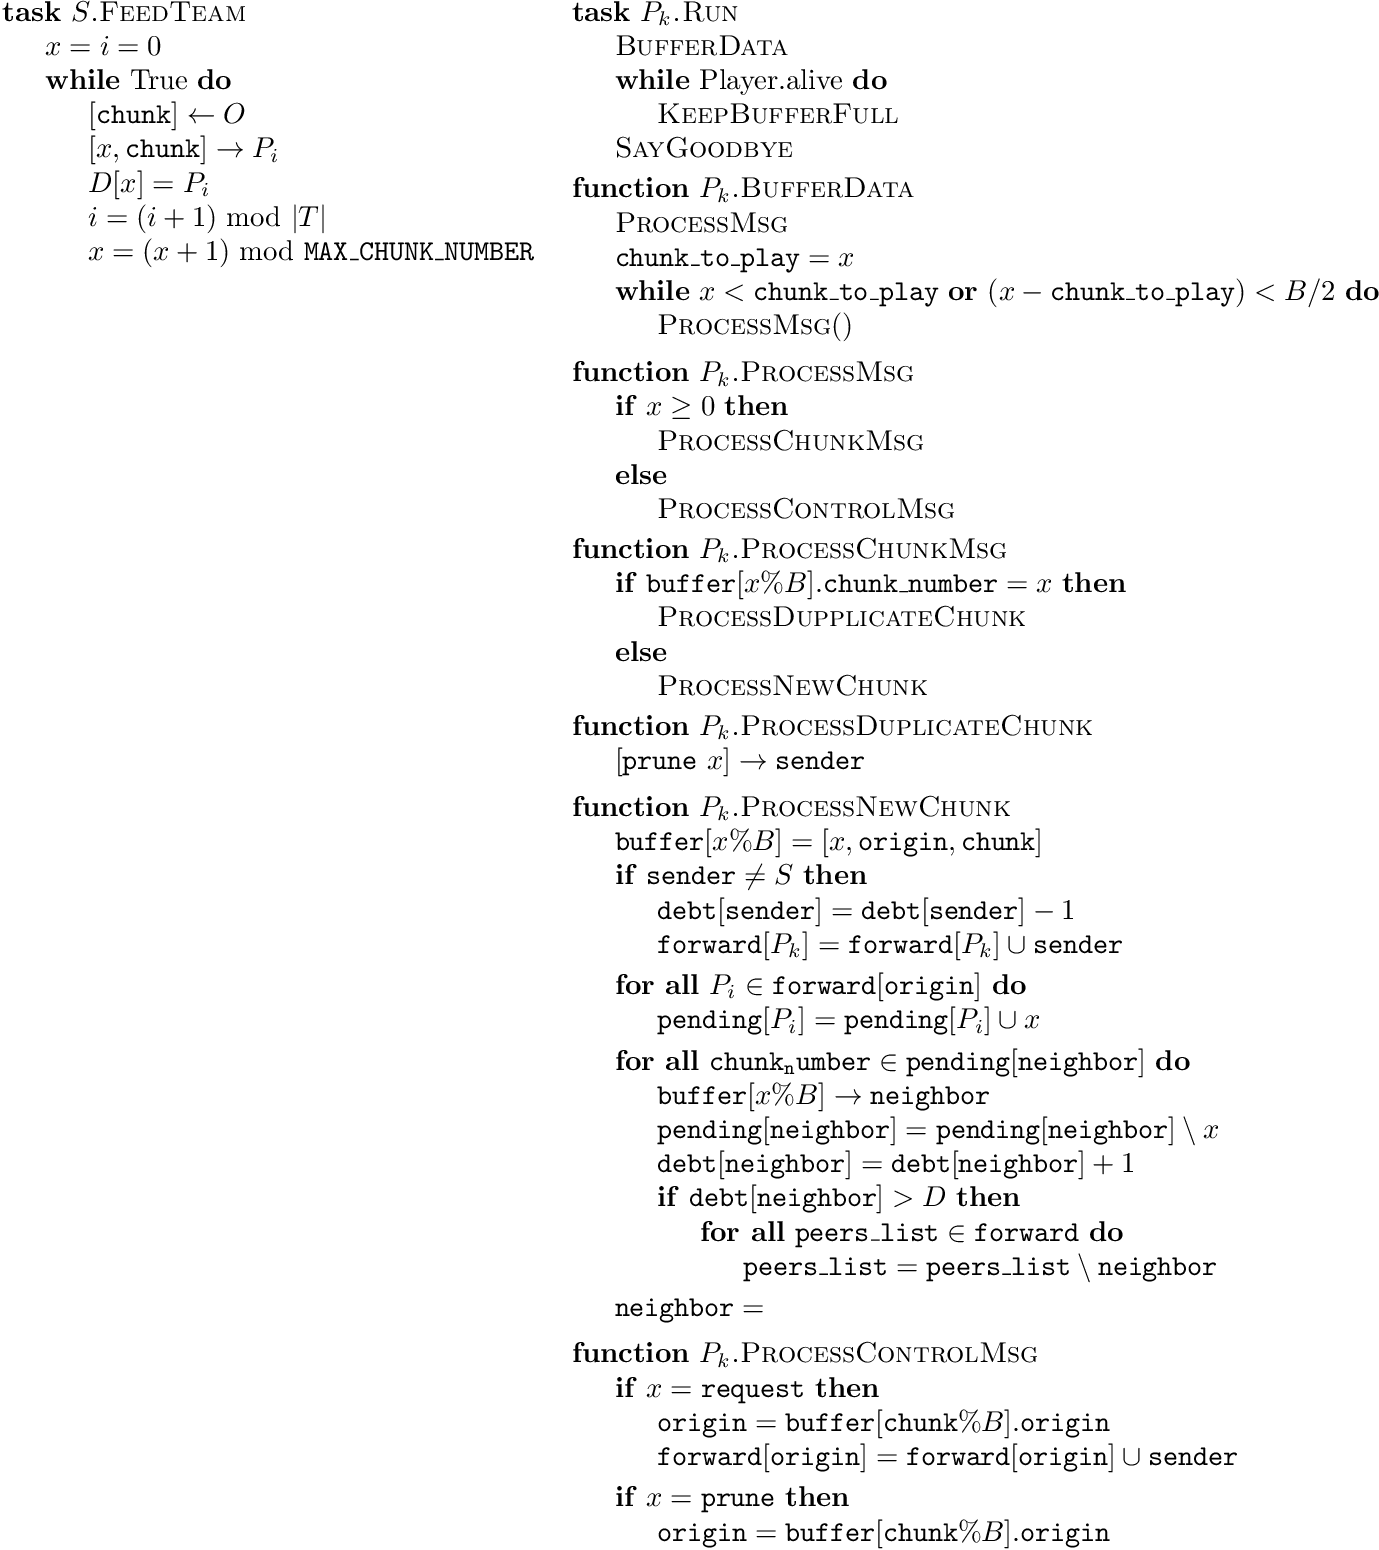
\includegraphics[width=0.75\textwidth]{chunk_generation_and_flooding} \fig{100}{3cm}{chunk_flooding} \caption{Chunk
  flooding at peers.\label{fig:chunk_flooding}}
\end{figure*}
When a peer $P_k$ receives a chunk from $P_i$, $P_k$ floods the
chunk to $T^k \setminus P_i$, using a prioritized round-robin
schema (see Fig.~\ref{fig:chunk_flooding}). Besides, if
it is a duplicate chunk, $P_k$ sends to $P_i$ a
$[\mathtt{NRFCF}~P_l]$ ($\mathtt{N}$ot $\mathtt{R}$elay
$\mathtt{F}$uture $\mathtt{C}$hunks $\mathtt{F}$rom) message, where
$P_l$ is the origin peer of the duplicate chunk. Thus, only
the first neighbor $P_i$ to send to $P_k$ a chunk
``originated'' at $P_l$ will do that in the future, at least
that $P_k$ revokes this routing information by sending a
$[\mathtt{RFCF}~P_l]$ ($\mathtt{R}$elay $\mathtt{F}$uture
$\mathtt{C}$hunks $\mathtt{F}$rom) to one or more (possibly the rest
of) peers of $T^k$.

As it has been said before, peers prioritize the flooding of the
chunks they relay by sending first the chunks to those neighbors that
are more supportive. To achieve that, every time $Pj_k$ sends a chunk
to $P_l$, $P_k$ runs $\mathtt{debt}[P_l] = \mathtt{debt}[P_l]+1$, and
$P_l$ runs $\mathtt{debt}[P_k] = \mathtt{debt}[P_k]-1$ (see
Fig.\ref{fig:}). Basically, these tables maintain a ``debt'' of chunks
between evey pair of neighbor peers. In ideal circunstances, debs
should be $0$. Debs are clipped to
$\pm\mathtt{debt}_{\text{max}}$. Obviously, a high supportivity means
a low debt, and viceversa.

\begin{comment}
In each round, peers check if a chunk have been received from the rest
of peers of the team (${\cal P}_k\in {\cal T}_j)$). If not, peers send
a $[\mathtt{propagate}~{\cal P}_i]$ to one or more (possibly
to the rest of) peers of the team, where ${\cal P}_i$ is the origin peer
of the missing chunk. At this point, the process continues as
described in Section~\ref{dbs:chunk_flooding}.
\end{comment}

\begin{comment}
For each ${\cal P}_k\in N({\cal P}_i)$, ${\cal P}_i$ checks if a chunk
has been received from ${\cal P}_k$. If ${\cal P}_i$ detects that
${\cal P}_k$ has not sent a chunk to it during $L$ consecutive rounds,
performs $N({\cal P}_i) = N({\cal P}_i)\setminus{\cal P}_k$, and stops
sending to ${\cal P}_k$ more chunks.
\end{comment}
\begin{comment}
computes a
``chunk-debt'', denoted by $d({\cal P}_k)$, that is incremented each
time a chunk is received from ${\cal P}_k$ and decremented each time a
chunk is sent to ${\cal P}_k$. If ${\cal P}_i$ verifies that $d({\cal
  P}_k)>D$ (the maximum debt), then ${\cal P}_i$ considers that ${\cal
  P}_k$ is unable to communicate with it, performs $N({\cal P}_i) =
N({\cal P}_i)\setminus{\cal P}_k$, and stops sending to ${\cal P}_k$
more chunks.
\end{comment}


%When peers receive chunks from their splitter, they must flood them to
%their neighbors until the chunks are broadcasted to the whole team
%(Fig.~\ref{fig:chunk_generation_and_flooding}). Lets suppose that
%${\cal P}_k$ receives a chunk. In the case the sender is its splitter,
%${\cal P}_k$ floods the chunk to $N({\cal P}_k)$. However, if the
%sender is a peer ${\cal P}_m\in N({\cal P}_k)$, ${\cal P}_k$ adds
%${\cal P}_m$ to $N({\cal P}_k)$ if ${\cal P}_m$ is a new neighbor, and
%forwards the chunk to the rest of its neighborhood ${\cal P}_n\in
%N({\cal P}_k)\setminus{\cal P}_m$ if ${\cal P}_k$ is in the shortest
%between ${\cal P}_n$ and the origin peer ${\cal P}_i$ of the relayed
%chunk. This will be true if ${\cal P}_k$ is the gateway of ${\cal
%  P}_n$ to go from ${\cal P}_n$ to ${\cal P}_i$. Therefore, a flooding
%with prunning based on shortest path routing is used.
